% Chapter Template

\chapter{Development and Discussion} % Main chapter title

\label{Chapter4} % Change X to a consecutive number; for referencing this chapter elsewhere, use \ref{ChapterX}

%----------------------------------------------------------------------------------------
%	SECTION 1   % TARGET 6000 WORDS IN THIS CHAPTER
%----------------------------------------------------------------------------------------

\section{Overview}

The first revision of the case prototype, PCBs and hardware-implimented accessibility features are presented in this chapter.
This chapter first covers the initial designs before moving onto the tangible 3D-printed prototypes with an analysis of the outcomes of these prototype.
The chapter then goes into detail about the design process, including how certain aspects align with the seven design principles, or support Digital Sovereignty as well as justifications as to why a specific approach was selected over potential alternatives.

%----------------------------------------------------------------------------------------
%	SECTION 2
%----------------------------------------------------------------------------------------

\section{Initial Concepts}

At the initial stage of planning, multiple approaches to the MEGAphone chassis were conceptualised before making a final selection. 
Two of these designs incorporated ‘stands’ to prop the device up in order to minimise physical effort from the user, as well as all designs featuring a curved or ridged design to accommodate comfortable device holding for a large range of hand grip sizes. 
It is important to note that these initial designs do not account for the notable features of the final prototype, such as the EZ access keys or the large rocker switch array.
Those features are discussed in detail in section 3 and section 4, as they appear later in the development process.
Each of the initial designs are outlined in the following sub-sections.

%-----------------------------------
%	SUBSECTION 1
%-----------------------------------
\subsection{Design One}

% LIST PROS AND CONS OF EACH DESIGN
% PERHAPS RANKING SYSTEM, EXPLAIN WHY DESIGN 3 WAS CHOSEN

Design ‘One’ as named was the first concept to be sketched using LibreCAD software.
The tapered design around the ports is intented to illustrate clearly to the user where all device ports are, in support of design principle four. 
It is worth noting that ideally, all ports should be oriented the same way to further support that design principle, however, as discussed in chapter 1, these are the constraints set for the project.
The addition of a device stand is intended to support design principle six, in that users can set their device down in a viewable orientation as opposed to potentially having to hold the device for extended periods of time.
In hindsight, most of this design’s features are quite mundane in that while they account for all major ports and include a device stand to prop it up, in terms of the ergonomics, there are very few stand-out features. 
One thing that can be noted is that the case is compact with curved profile on either side where the user’s hands are expected to rest which is once again .

\begin{figure}[hbt!]
\centering
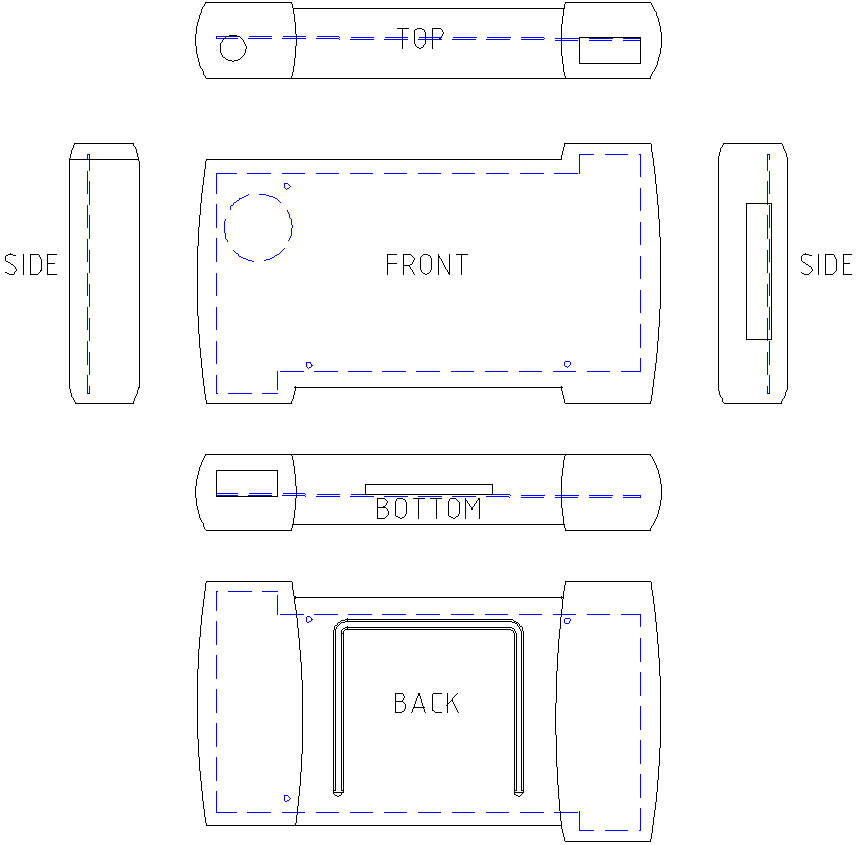
\includegraphics[width=10cm,height=10cm,keepaspectratio]{Figures/design1_sketch.png}
\caption{This is a sketch of the first concept design drawn to scale of the PCB}
\label{fig:Design_1}
\end{figure}

%-----------------------------------
%	SUBSECTION 2
%-----------------------------------
\subsection{Design Two}

Following design principle three, the second design was intended to mimic a video game controller in order to conform better to the hand and give users a more intuitive layout in regards to the orientation of the device when in use. 
This concept inhabits this trait arguably to the highest degree in that most users would familiar with a somewhat modern gaming controller conventions and will immediately understand how the device is meant to be held (design principle three).

\begin{figure}[hbt!]
\centering
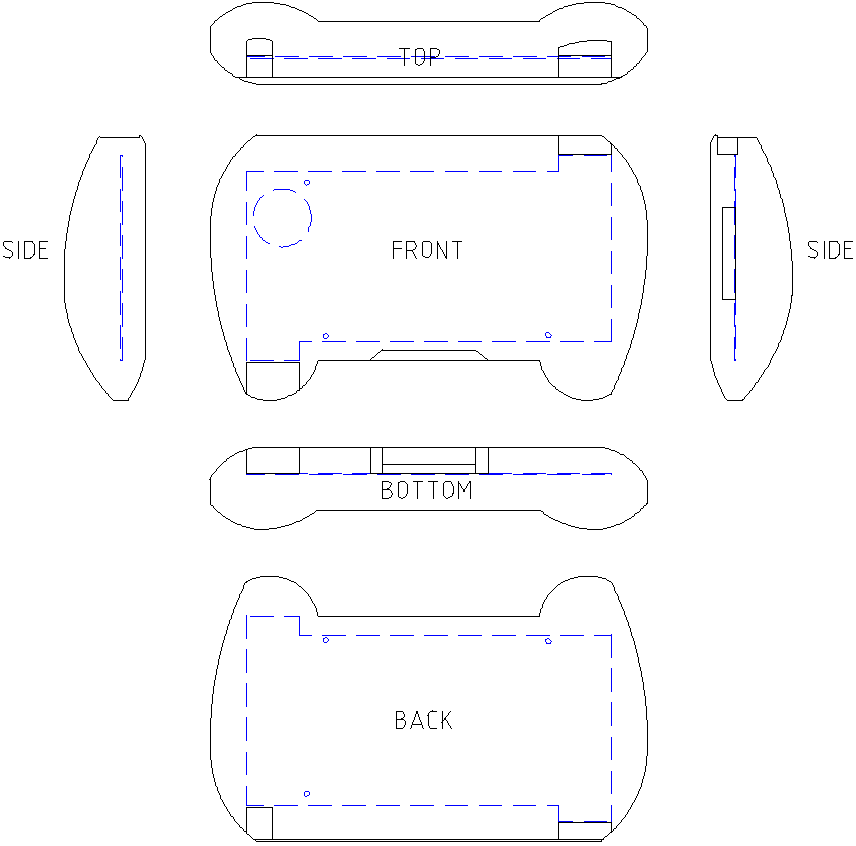
\includegraphics[width=10cm,height=10cm,keepaspectratio]{Figures/design2_sketch.png}
\caption{This is a sketch of the second concept design drawn to scale of the PCB}
\label{fig:Design_2}
\end{figure}

%-----------------------------------
%	SUBSECTION 3
%-----------------------------------
\subsection{Design Three}

There were a few factors that made this design the final candidate in which to base the main deliverable of this project.
This approach uses handgrips to subconciously hint to the user the correct orientation to hold the device, which like design two, supports design principle three.
The use of a stand to prop the device up for extended periods of time reduces the amount of effort from the user, therefore reducing fatigue much like design one.
For these reasons, this was the design in which the project is based.

\begin{figure}[hbt!]
\centering
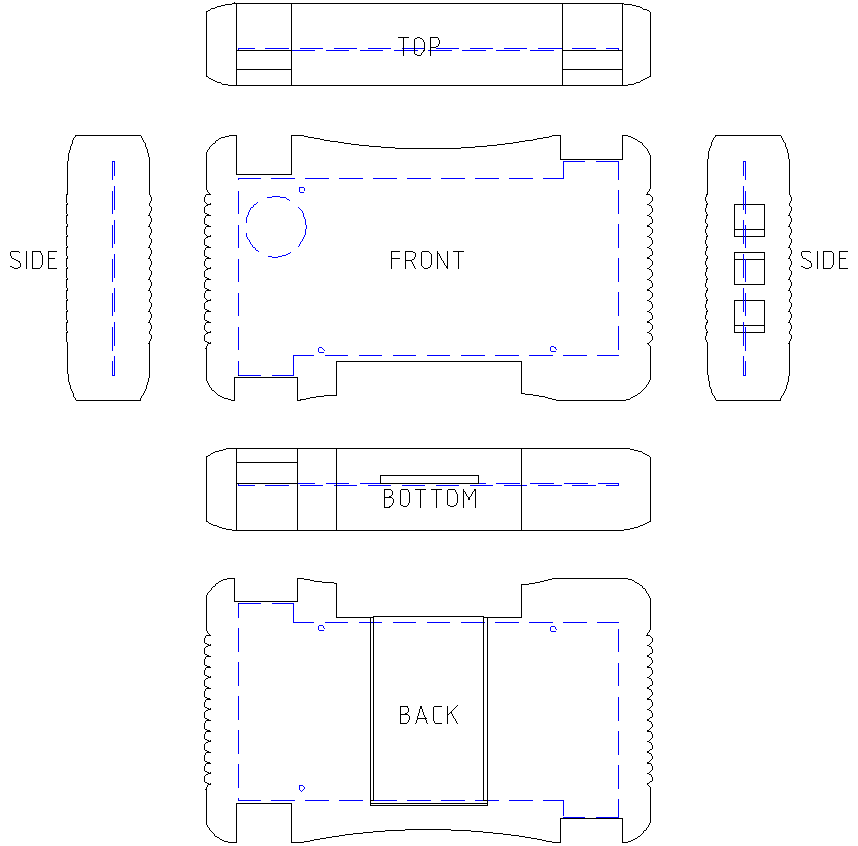
\includegraphics[width=10cm,height=10cm,keepaspectratio]{Figures/design3_sketch.png}
\caption{This is a sketch of the third concept design drawn to scale of the PCB}
\label{fig:Design_3}
\end{figure}

%----------------------------------------------------------------------------------------
%	SECTION 3
%----------------------------------------------------------------------------------------

\section{First Revision}
This section provides a broad view over the design process with a 'timeline' based approach, making note of the problems and solutions regarding 3D-printed prototypes.
Detailed evaluations of specific design features are provided in section 4.

%-----------------------------------
%	SUBSECTION 1
%-----------------------------------
\subsection{First 3D-print}

There was a significant issue that was overlooked with the first 3D-printed prototype in that the thought behind orientation of components was flipped.
Electronic components (including connectors) needed more space underneath in order to fit comfortably and the design up until that point had not properly accounted for it.
The biggest issue was that the device ports were initally not thought of in the correct orientation.
The orientation of these ports is very important as this dictates how much volume each of the two main case components takes.
To rectify this issue, %%FIX THIS

% so explain the process of rectifying this issue, map out the impacts and how they are resolved
% also add in that 0.15mm print resolution was used, not perfect as the project was very precise on top case in some parts, such as buttons, hence this should be done at higher resolution which means longer print time or silicone injection mould as a likely stronger, neater alternative

%-----------------------------------
%	SUBSECTION 2
%-----------------------------------
\subsection{Second 3D-print}
//

%-----------------------------------
%	SUBSECTION 2
%-----------------------------------
\subsection{Final 3D-print}
//

%----------------------------------------------------------------------------------------
%	SECTION 4
%----------------------------------------------------------------------------------------

\section{Design Features}

The following section covers the development of all specific aspects of the accessible MEGAphone chassis as well as the accompanying hardware such as buttons or hinges.

%-----------------------------------
%	SUBSECTION 1
%-----------------------------------
\subsection{CAD Sketch}

The first stage of design after the initial concepts was the CAD sketching stage.
This was approached by beginning with a front view of the sketch where users would typically interact with the device, however just the outline was extruded outwards in order to create a tangible object in which to mold and add features later on in the process.

%-----------------------------------
%	SUBSECTION 2
%-----------------------------------
\subsection{Hand Grips}

The first stage of design after the initial concept sketches intended to use rubber grips on both sides of the device featuring a ridged pattern.
However, this concept was removed in favour of a ridges that resemble the size and shape of human adult fingers to more intuitively direct the user to hold the device in the correct fashion as the third design principle.
Another aspect that was considered since the early stages, while less obvious in the final product due to the curved nature, was the introduction of rounded corners as this would minimise hazards to the user.
This was also the case with other edges of the device, in that they were filleted at 1.5mm to remove the sharpness of the device.
Doing adds to the softness from the device and makes it arguably safer for users.

% This was after receiving feedback from my supervisor following an initial design (show design, before and after).

%-----------------------------------
%	SUBSECTION 3
%-----------------------------------
\subsection{Rocker Switches}

A major issue that was identified from the start with the second revision PCB was that placement and size of switches made it difficult to access.
Larger rocker switches were chosen to be placed on the front surface above the screen as this is in full visability of the user during use.
These switches relate to the security draw of the MEGAphone device, with insecure modules including, WIFI, bluetooth, two 4G modems, MEMS mics, LoRa radios and the FPGA serving as the central processing unit of the device.

The orientation of switches was completely intentional; for easier access for those with limited motor function or even without fingers, having the switches flip vertically would ensure that users are far less likely to flip wrong switch.
As well as this, the placement of these switches, above the display and away from other buttons on the device ensures that they do not interfere with the operation of the device.
Design principle one and three are satisfied by these rocker switches as they make the security features of this device easily available and the ON/OFF state of wireless modules is made abundantly clear (also supported by LED lights).

An earlier design incorporated the use of standoffs in the design in which to mount the PCB for the switches which was additionally included in the PCB design (view section 4.4). %fix this
This was however later removed in support of design principle three in an effort to reduce undesired complexity.
Additionally, it was considered completely unnecessary as when soldered to the switch contacts, the PCB would hold in place, securely and without issue.
On top of this, the rocker switches are placed in from the outside of the device in a press fit and due to their flat extended base at the 'top', pushing down on the switches beyond a certain point is not possible.

%-----------------------------------
%	SUBSECTION 4
%-----------------------------------
\subsection{Jellybean Switch}

The Jellybean switch sourced for this project interfaces with the device using a 3.5mm Audio Jack connector, a standard feature with accessible switches.
This is very much in the spirit of Microsoft's Xbox Adaptive Controller\cite{adaptive} in that it supports the same standardised connector with the intention of allowing a greater degree of adaptiblility or freedom for the users needs.
Another benefit of implementing Jellybean switch accessibility is that it supports the second design principle as it accommodates users who may have great difficulty using the relatively small buttons (which are existing constraints linked to the PCB) or however less likely, the EZ access keys.
Given that it is a single digital input device, hardware-implemented accessibility (view section 6) capable of easily communicating with this device was relatively simple to implement. 
The second revision PCB during commencement of this project did not feature a working 3.5mm Jack connector, therefore, based on this knowledge, the 9-pin DSUB port of the device was hijacked as a single digital input under pin 7 for the Jellybean switch. 
The PCB ‘adapter’ created for this purpose is discussed in section 4.4.
This uses the same pin as the fire button on a retro Commodore64 Joystick controller, hence, integration into the MEGA65 operating system would be straightforward.

\begin{figure}[hbt!]
\centering
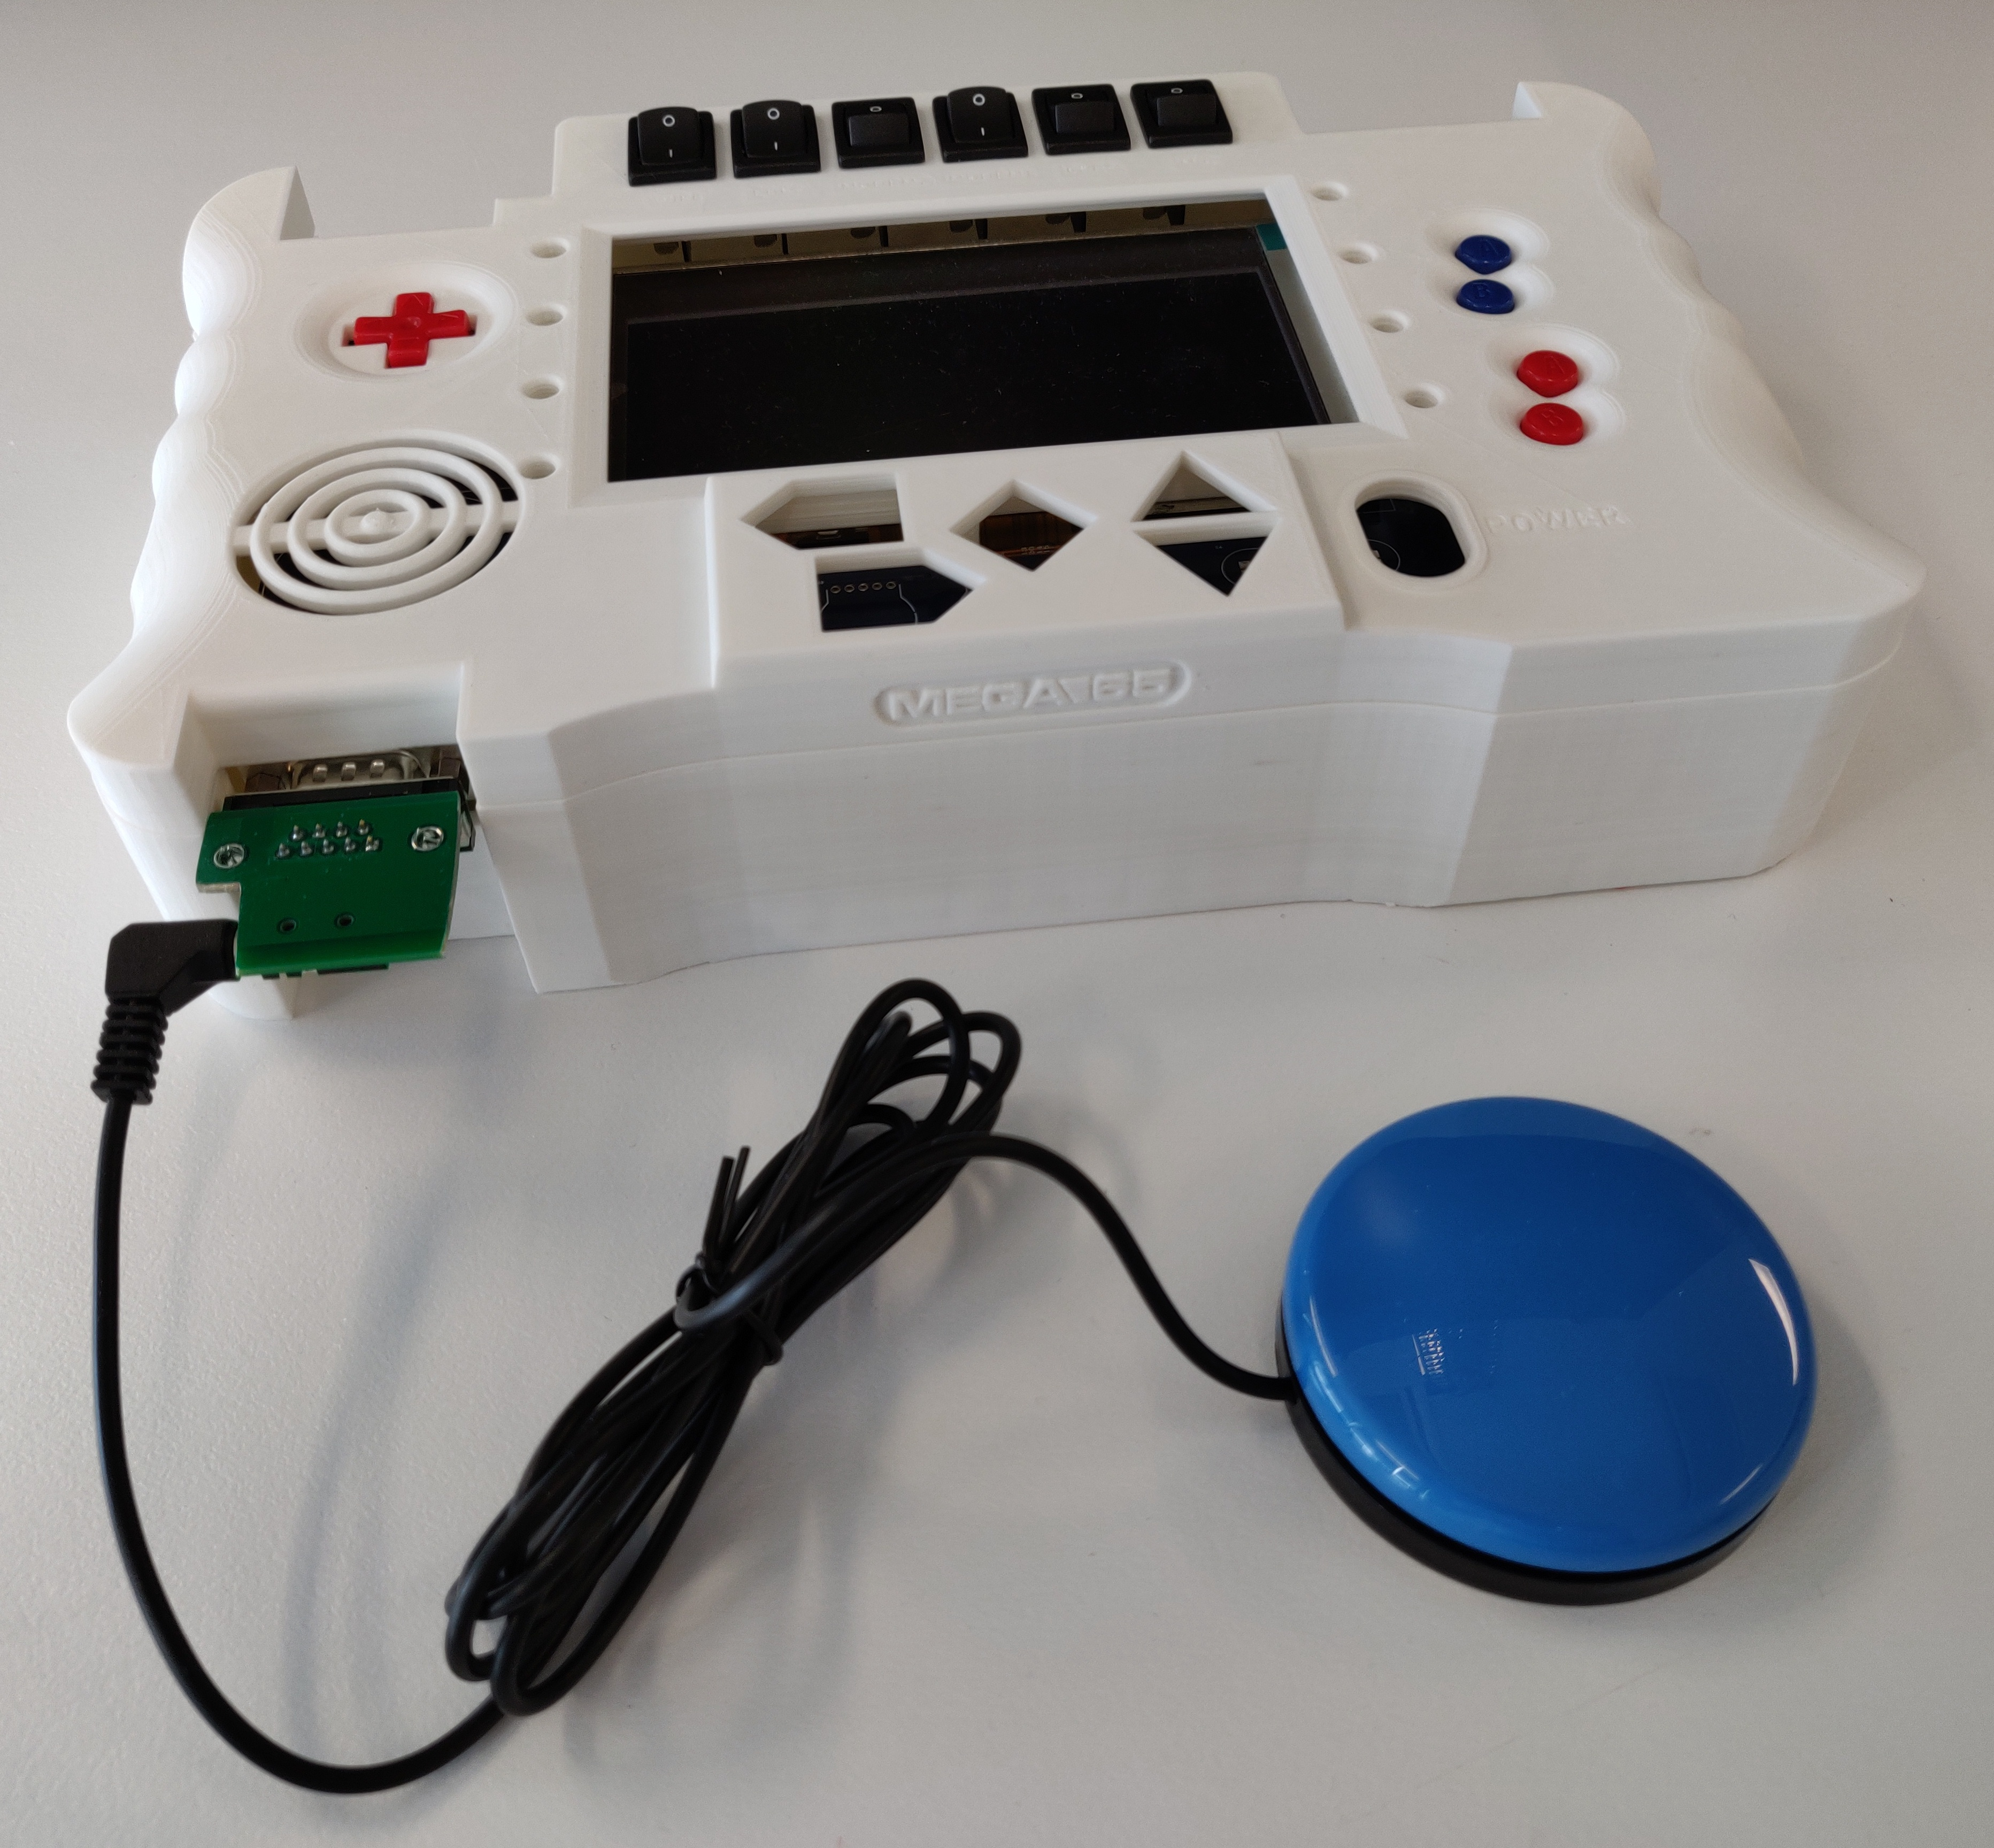
\includegraphics[width=10cm,height=10cm,keepaspectratio]{Figures/jellybean.jpg}
\caption{This is a physical example of how the Jellybean switch interfaces with the device during development}
\label{fig:Jellybean}
\end{figure}

%-----------------------------------
%	SUBSECTION 5
%-----------------------------------
\subsection{Recessed Buttons}

% talk about recessing the buttons so that if the device is dropped, minimal/no accidental button presses are registered
One concept that improves the ‘quality of life’ of this product was the addition of recessed buttons.
There are potential situations where the device might be accidentally dropped and unintended button presses may be recorded where the addition of recessed buttons avoids or at least significantly reduces the risk of this situation.
This feature also supports design principle five in that it minimises risks of unintended actions such as accidental button presses, which in this case would be if the user drops the device.

This feature is designed around another existing constraint in that the PCB uses buttons that were repurposed from spare Gameboy Advance parts. %%check this!
On the first prototype print, while allignment on the main MEGAphone PCB was correct, there was an issue regarding the clearance of the button cutout as well as the positioning of slots to hold the buttons in the correct orientation.

%-----------------------------------
%	SUBSECTION 6
%-----------------------------------
\subsection{Battery}

Due to the addition of a new proposed 7.4V 5000mAH Lithium-Ion battery, considerations had to be made in regard to placement within the MEGAphone device chassis.
There were two potential approaches to this issue in that the battery could either be placed internally within case along with the electronics, or 'externally' on the 'bottom' of the device with a separate cover that could be screwed on to hide the battery like what might be found on an RC Car controller for example.

The approach that was chosen was to have the battery be housed within the case along with the PCBs with he second approach ultimately not being chosen for a number of factors.
While the intention of the device is certainly not to be waterproof, there was some desire for the device to protect against light rain, which meant 'sealing' up electronic components at least to the best ability.
There is also the concern that the 'bottom' of the device already makes the most of the available space by housing the device stand (view section 3.8) and the solar panel array and therefore the only plausible solution would be to remove the solar panels every time the user requires access to the battery.
As the solar panels would most likely be stuck down, this would make removing the battery a more painful process.
Having the battery be inside within the same compartment as the PCBs, ensures simplicity due to having less parts, provides more protection from the elements and as per design principle five, protects users against potential hazards under normal use.

The battery housing was labelled for clarity and placed assymetrically to the user's left side due to the location of the bulky FPGA board on one side of the MEGAphone PCB.
This was a change that was addressed in a later stage of development, as the original intention was to place the battery be placed symmetrically on the device as this is best for weight distribution.
In order to not contribute too significantly to the thickness of an already objectively thick device, this was deemed the only reasonable solution to that problem.

%-----------------------------------
%	SUBSECTION 7
%-----------------------------------
\subsection{Device Stand}

% thoughts behind the device stands, how they were conceptualised and why it was approached in such and such way; having two stands on either side adds to stability of the device as opposed to the original idea of having one stand in the middle, which also leaves space for solar panel in the middle
Originally the approach was to have a single stand oriented in the middle of the device where users could extend it out as they need.
However, having two stands on either end of the device has multiple advantages in that doing so increases the stability of the device, as well as giving ample space in the centre to place one or multiple solar panels depending on the available space (discussed in section 3.8).
The mechanism in which to extend and 'lock' the stand in place had the potential to be approached from a number of different angles.

The approach that ended up in the final prototype was to have a sliding mechanism that users could 'slot' in first, followed by a clearance fit in which the stand can rotate around a cylindrical 'mounting' point.  %%show pictures of all this!!
At the opening of the stand where it is expected to assemble with the cylindrical base of the 'mounting' point, a location fit is used, meaning that the user must use mild force in order to get the stand to 'snap' into place.
This ensures that the stand does not fall off the device unintentionally when in normal use.
The aforementioned sliding mechanism slots into two notches which holds the stand in either a horizonal position, flush with the MEGAphone chassis, or an extended position at about 45 degrees so that the device can be propped up under an extended use case.

An alternative that was considered that would have proven to be effective, was to have the cylindrical 'mounting' point in which to revolve the stand, be a part of the stand.
This would mean that the %%FIX THIS

%%add trigonometric function to determine angle of stand 'foot'

%-----------------------------------
%	SUBSECTION 8
%-----------------------------------
\subsection{Solar Panels}

% choice of solar panels, discuss potential options and why a specific one was chosen, do a table comparison of available panels and again explain the power output and cost etc.
Giving users more ways to charge their device plays heavily into the Digital Sovereignty aspect of this project as this provides a platform in which to harvest energy to power the device without the need for an energy infrustructure.
This is something that Gardner-Stephen, in one of his CCC talks, lists as one of the six freedoms to protect against the 'Digital Winter' which Gardner-Stephen refers to as the "situation where the freedoms to create and [innovate] digital systems will become impossible or highly limited" due to a number of reasons listed such as totalitarian governments or failure of critical infrustructure"\cite{freedoms}.
A number of solar panels from two suppliers (Digikey, Mouser) were analysed based on cost, size and energy output for a designated area set out on the MEGAphone case at 125mm by 140mm, collated in figure X.

\begin{center}
    \begin{tabular}{ |c|c|c| } 
    \hline
    cell1 & cell2 & cell3 \\
    \hline
    cell1 & cell2 & cell3 \\ 
    \hline
    cell1 & cell2 & cell3 \\ 
    \hline
    cell1 & cell2 & cell3 \\
    \hline
    \end{tabular}
\end{center}

\begin{figure}
    \caption{An analysis of various solar arrays and their suitability to a designated space on the MEGAphone chassis}
    \label{fig:DesignPrinciples}
\end{figure}

%-----------------------------------
%	SUBSECTION 9
%-----------------------------------
\subsection{Device Strap / Key-chain}

% talk about process of designing this feature, how original design changed in favour of larger slot/strap for easier carry
The thought behind the key-chain feature of the device was to be able to clip it to something or alternatively fix items to it, and while this feature did see an appearance in an early prototype, it was later adapted into a 'housing' for an arm strap, to allow for easier carrying as this was considered to be more useful.
The reasoning for the original implementation of a key-chain feature was to give users the option to strap the device to their hand in cases where they might have a weak grip strength, minimising the risk of dropping the device and supporting the second design principle.
Due to that feature not having many other practical applications in terms of hanging items off of it, the introduction of a much larger opening to integrate a carry strap would better benefit design principle six as it would distribute the weight of the device more evenly when carried.
This would still however allow the option for a hand strap, therefore not eliminating that feature entirely.
Another consideration was the addition of an extra notch, added to lock into the top part of the case and re-enforce the strength as the entire weight of the device would otherwise be supported by one end of the slot. %%revise, find better name for 'slot'
The device weights a little under one kilogram, even at that weight it makes sense to distribute the weight more evenly.

%-----------------------------------
%	SUBSECTION 10
%-----------------------------------
\subsection{Easy Access Keys}

The easy access keys or 'EZ Keys' were inspired by the 'Nav Keys' developed by Storm Interface [source] which feature an array of easily distingishable keys which were inspired for this adaptation.
These keys benefit from being easily perceptible which envelops the forth design principle, due to each button not only having a unique colour and shape but also a distinct tactile feel when a button is pressed.

The EZ Keys were first approached as an extension of the device as this would free up a lot of the limited space available.
This would mean making a separate housing and having the device plug into the 9pin DSUB port similarly to how the Jellybean switch (see section 3.4) would interface with the device.
It was ideal for the array of buttons to be integrated into the device as this ensures that the full extent of accessibility is available from the moment the device is picked up.

Due to the height requirement of the MEGAphone PCB, there was very little space to attach a slave PCB to allow button functionality, hence one of the reasons why there is an elevation in the button housing.
The second reason for there being an elevation in the EZ key setup is due to the desire to make it more perceptible (design principle four) to users as the position of the power button nearby meant that it would be important to ensure that users do not accidentally press the wrong button (design principle five).
Additionally, there needed to be enough depth so that the PCB could be screwed into place comfortably, elevated slightly above the main MEGAphone PCB as there would be an overlap due to the size and shape of both PCBs.

An issue that came up in the first prototype print is that the keys did not have enough clearance to actuate without resistance, also in common with the A, B and directional buttons.
This was fixed in an update by extending the width of the button cutouts by approximately 0.3mm as this would also theoretically align with the 0.15mm print resolution. % check this

% FIXED AB AND DIRECTIONAL BUTTON SIZE CLEARANCE, ALSO EZ KEY CLEARANCE
% FIXED ALIGNMENT OF THROUGH HOLE

%-----------------------------------
%	SUBSECTION 11
%-----------------------------------
\subsection{Ventilation} %PROBABLY CHAPTER 5

% device only uses about 1-2W of power, FPGA using 0.2W
% Not necessary in final design but add images of version with vents
Thermal management is a concept that came up later in the process as the MEGAphone device is a low power device by mobile device standards.
In its entirety, the device uses approximately 1-2W of power with the heart of the device, the FPGA, using about 0.2W of power.
This yields very little thermal output with the more notable power drawing components being the 110db speaker [source] and full colour 480p display [source].

%-----------------------------------
%	SUBSECTION 12
%-----------------------------------
\subsection{Potentiometers}

% Slide pot better than thumb wheel pot, explain about physical effort etc.
%% LIKELY GOING IN CHAPTER 5
The potentiometer feature used to control aspects such as speaker volume was a feature that was omitted from the final design due to another more important requirement being the implimentation of EZ keys.
This is a feature that can be implemented by other means such as through the EZ keys themselves and therefore a prototype without this would not be a major issue.
The best solution for this would be to employ an array of sliding potentiometers to control any desired functions such as volume control, as pertaining to design principle six, would be the easiest in terms of the amount of effort that users have to extert.
Any potentiometer that is too small or requires a twisting motion would be more difficult for some users, such as elderly users with a weaker grip strength.

%-----------------------------------
%	SUBSECTION 13
%-----------------------------------
\subsection{Port Access}

Port access was intentionally designed to have no case material on the top and bottom of the device minimise interference with the plugging in of various peripherals, supporting design principle seven.
These ports are all labelled, explaining in one word the purpose of each port to make it abundantly clear to the user.

An issue that was faced in the original prototype was in regard to the orientation of the port cutouts that were placed on the display side of the PCB.
This was rectified by extending out the bottom chassis component with the port cutout on that side so that it would match up with the true orientation of the ports. %expand on this later with images

%-----------------------------------
%	SUBSECTION 14
%-----------------------------------
\subsection{Threaded Inserts}

An important aspect of this deliverable is to have a method of securing all parts in place as well as being easily accessible to users who which to repair or modify certain aspects.
This meant that using a 'pentagon star' screw[REF] would not have been a reasonable choice as it would make repair or modification more difficult, as users would typically not have the suitible screwdriver for that job.
Naturally, this would all be fastened using 'phillips head' screws as these are widely considered the most common screw head type aside from 'flat head' screws.

These constraints were already set out for the MEGAphone PCB in that there are holes in certain parts of the case for this exact purpose.
However, an issue that had to be addressed was the placement of certain components on the PCB and their vicinity to these 'mounting' points.
In particular, one of the MEMs mics, some resistors and transistors were placed closer to this mounting point than what would've been ideal and for this reason, certain parts of the mounting supports were trimmed around these obstacles.

The alternative that would acheive the same outcome would have been to 3D print solid standoffs and use self-tapping screws in order to securely fasten the device.
This option is however more unreliable as it requires user guided input, a reasonably soft material to be effective and most importantly would require a 100 percent 3D infill, almost doubling the overall print time.

A third option that was diregarded would have been to 3D print the threads, which at a 0.15mm print profile, would have left much room for error considering that this project requires considerably small M3 screws to remain compliant with the constraints of the MEGAphone PCB.

The choice to use threaded inserts for this project was due to its reliability, in that the threads must be consistent due to strict manufacturing standards.
Another reason why they were a solid choice was due to the fact that they are readily available from any hardware store, making sourcing of this component very convienient.

%-----------------------------------
%	SUBSECTION 15
%-----------------------------------
\subsection{MEGAphone PCB}
A new MEGAphone PCB was built up for this project, that being soldering of the surface-mounted components and through-hole components.
For the most part, very little changes were made from the original two second revision PCBs, and while one of those two could have certainly been modified to fit these new parameters, external factors meant that those PCBs could not be accessed.
As discussed briefly in section 4.3, the changes made included the addition of rocker switches and therefore the removal of the much smaller slide switches. %%add sources
As well as this, the previously used thumbwheel potentiometers were intentionally left out not only due to the potential to interfere with the EZ access keys PCB due to the very little clearance of 4mm but moreso as the desire is to hijack this for testing slide potentiometers in the future.
The implementation of slide potentiometers significantly benefits the usability of the device and while the thumbwheel design works much in the same way, there is currently no realistic way to access it without moving or removing the EZ access key feature which can theoretically be used for the same function by reconfiguring the FPGA.
Not to mention their horizonal placement would mean that they only make sense to be placed on the 'bottom' of the device in the same space as the MEGA65 logo, which from an intuitive use standpoint (design principle three), is not ideal.

%----------------------------------------------------------------------------------------
%	SECTION 5
%----------------------------------------------------------------------------------------

\section{PCB Design}
This section discusses the process in designing the supporting PCBs for this project.
% explain workaround for previous button layout, using slave boards with tactile switches as well as choice behind contact pads instead of connectors to save space

%-----------------------------------
%	SUBSECTION 1
%-----------------------------------
\subsection{Rocker Switch PCB}

The PCB designed to organise the routing of power to the array of rocker switches originally had the intention of interfacing with the main PCB through a connector of some sort.
With space being a limited factor, an alternate solution was carried out.
The introduction of 'mounting' pads to serve as a soldering point for the wires would allow them to be comfortably routed to the main PCB.

An issue with the footprint that was observed after sourcing these parts, was that there was not enough clearance for the pins to 'slot' through.
The approach was to file down the pins on the rocker switches individually so that they would fit, which was not an issue in regards to current as the whole device runs on about 1-2W, with a rocker switch[REF] able to handle approximately 2kW of alternating current.
Filing down the PCB through-hole cutout would have made for a far worse alternative as there was potential for solder to not flow evenly due to damaging the solder mask. %double check this

During the case design process, having mounting points to hold the circuit board in place was implemented.
This was later removed as the switches mount very securely in their cutouts coming from a top-down orientation and so pressing in or flicking these switches would not put any stress on the PCB, unlike the EZ keys in section 4.2.
Doing so allows for adjustment if needed before soldering as well as less parts making the repair process easier if users need to replace or modify certain parts.

Clearance between the PCB and the main MEGAphone PCB was additionally very minimal and so the introduction of a bulky connector would make containment of this device far more difficult.
An alternative to this that would have proven effective and arguably neater in a final version would have been to employ the use of a low profile 'ribbon' style connector with separate wires that are thick enough to handle decent current as well as be indepenently wired to different areas of the MEGAphone PCB.
The reason why this was not chosen is because this deliverable is a proof of concept where the intention is for the MEGAphone PCB to be redesigned so that these rocker switches can be incorporated into the main design, therefore purchasing these connectors for this purpose would be ultimately wasteful.

%-----------------------------------
%	SUBSECTION 2
%-----------------------------------
\subsection{Easy Keys and Power}

The purpose behind the Easy Keys or 'EZ Keys' as otherwise referred to, was to give users a platform in which to interact with the MEGAphone device while being as clear and easy to use as possible.
Multi-coloured, multi-shaped keys are employed make things as unambiguous as possible which include, left and right (forward and backward), up and down, and a 'fire' or enter key.
This, as discussed in section 3.10, is inspired by the Storm Nav-pad[source], where a version has been acheived to a budget, for the purpose of prototype development. %check typing of nav pad

An important aspect of this device is to provide easy access to the power switch as turning the display on an off on this device is frequent due to not having automatic display toggle features.
This is intergrated into the device in the same manner as the easy keys, in that they work by momentarily pressing a tactile switch.
These tactile switches are wired directly to the GPIO expander linked to the FPGA on the MEGAphone PCB with the idea being that this new external PCB serves as an extension of the main board.

The placement of the pads used to wire the EZ Key PCB was deliberately chosen to be routed to the 'bottom' of the PCB as this would keep the profile of the PCB at a state that is less obtrusive to the rest of the device.
Placing the pads on the 'top' side of the PCB, much like the rocker switches, would have interfered with the space of the LCD display, hence was not considered to be a sensible solution.

%-----------------------------------
%	SUBSECTION 3
%-----------------------------------
\subsection{Audio Jack Adapter}

The audio jack adapter was designed to be a substitute for the original audio jack setup fully integrated on the MEGAphone PCB, which was unoperational at the time.
This PCB hijacks the fire pin of the 9-pin DSUB connector in order to 'imitate' a joystick fire button. 
Coupled with hardware implemented features in the FPGA, the MEGA65 OS should treat this input as a regular peripheral such as a joycon.

An issue that was faced during the course of development regarded the overall size and shape of the PCB.
This was not thought about correctly at the time of manufacturing as the PCB was too bulky on either side.
Additionally, due to the central placement of the audio jack input and the bulky Jellybean switch jack output, interfacing with this adapter was less than convienient.
To fix this, a nibbler was used to clip away at the edges to cut the board down to size, followed by a rough 80 grit sanding to smooth the edges somewhat.
Given that fibreglass particles are not good for health when inhaled, this was undertaken responsibly to ensure that these risks were avoided.

%----------------------------------------------------------------------------------------
%	SECTION 6
%----------------------------------------------------------------------------------------

\section{Software Accessibility}
% talk about keyboard accessibility, term ‘android accessibility encapsulation’ discuss this.
% Also mention program is working in parallel to the software ‘mimicking’ the c64 system so this is not a C program running on MEGA65 but rather VDHL, a hardware description language
Digital Sovereignty covers a broad context, where the overarching concept is about giving users control over their own data[source], where in this case, providing the MEGAphone device with accessible software features can be argued as achieving an extent of this project in that it places more control in the hands of the users.
On a different note, the keyboard 'software' accessibility aspect of this goes hand-in-hand with the Jellybean switch input (view section 3.4) as this is primarily what is used to control this feature, aside from the potential to implement this on an EZ key button by hijacking the same pin.
This is all hardware-implemented in the FPGA, with the intention of being completely transparent to the MEGA65 operating system.
This means that the accessible keyboard runs in parallel to the operating system and therefore should not 'see' the Jellybean switch, but instead treat it as if it were any peripheral, such as a Commodore64 joycon[source].
Due to the Jellybean switch being a simple digital input device, this made implementing this feature relatively straightforward.

% %-----------------------------------
% %	SUBSECTION 1
% %-----------------------------------
% \subsection{Accessible Keyboard Framework}
% //

% %-----------------------------------
% %	SUBSECTION 2
% %-----------------------------------
% \subsection{Accessible Interface}
% //

%----------------------------------------------------------------------------------------
%	SECTION 7
%----------------------------------------------------------------------------------------

\section{Summary}  %% TALK ABOUT THE DESIGN IN VARIOUS STAGES, PERHAPS IN A SECTION BEFORE FINISHING TO SHOW THE BIGGER PICTURE
//